\section{Overview}
\label{sec:overview}

Given a 3D model collection representative of a shape family, our goal is to compute probabilistic point correspondences and part segmentations of the input shapes (Figure \ref{fig:teaser}, left), as well as learn a generative model of 3D shape surfaces (Figure \ref{fig:teaser}, right). At the heart of our method lies a probabilistic deformation model that learns \rev{part templates} and uses them to compute fuzzy point correspondences and segmentations. We now provide an overview of our \rev{part template learning} concept, our probabilistic deformation model, and our generative surface model. 

\textbf{Learned part templates.} Our method computes probabilistic surface correspondences by learning suitable \rev{part templates} from the input collection. As \rev{part template}, we denote a learned arrangement of surface points that can be optimally deformed towards corresponding parts of the input shapes under a probabilistic deformation model. To account for structural differences in the shapes of the input collection, the \rev{part templates} are learned with a hierarchical procedure. Our method first clusters the input collection into groups containing structurally similar shapes, such as benches, four-legged chairs and office chairs (Figure \ref{fig:hierarchy}c). Then a \rev{template} for each semantic part per cluster is learned (Figure \ref{fig:hierarchy}b). Given the learned group-specific \rev{part templates}, our method learns higher-level \rev{templates} for semantic parts that are common across different groups e.g. seats, backs, legs, armrests in chairs (Figure \ref{fig:hierarchy}a). The top-level \rev{part templates} allow our method to establish correspondences between shapes that belong to structurally different groups, yet share parts under the same label. If parts are unique to a group (e.g., office chair bases), we simply transfer them to the top level and do not establish correspondences to incompatible parts with different label coming from other clusters.

\begin{figure}[t]
\centering
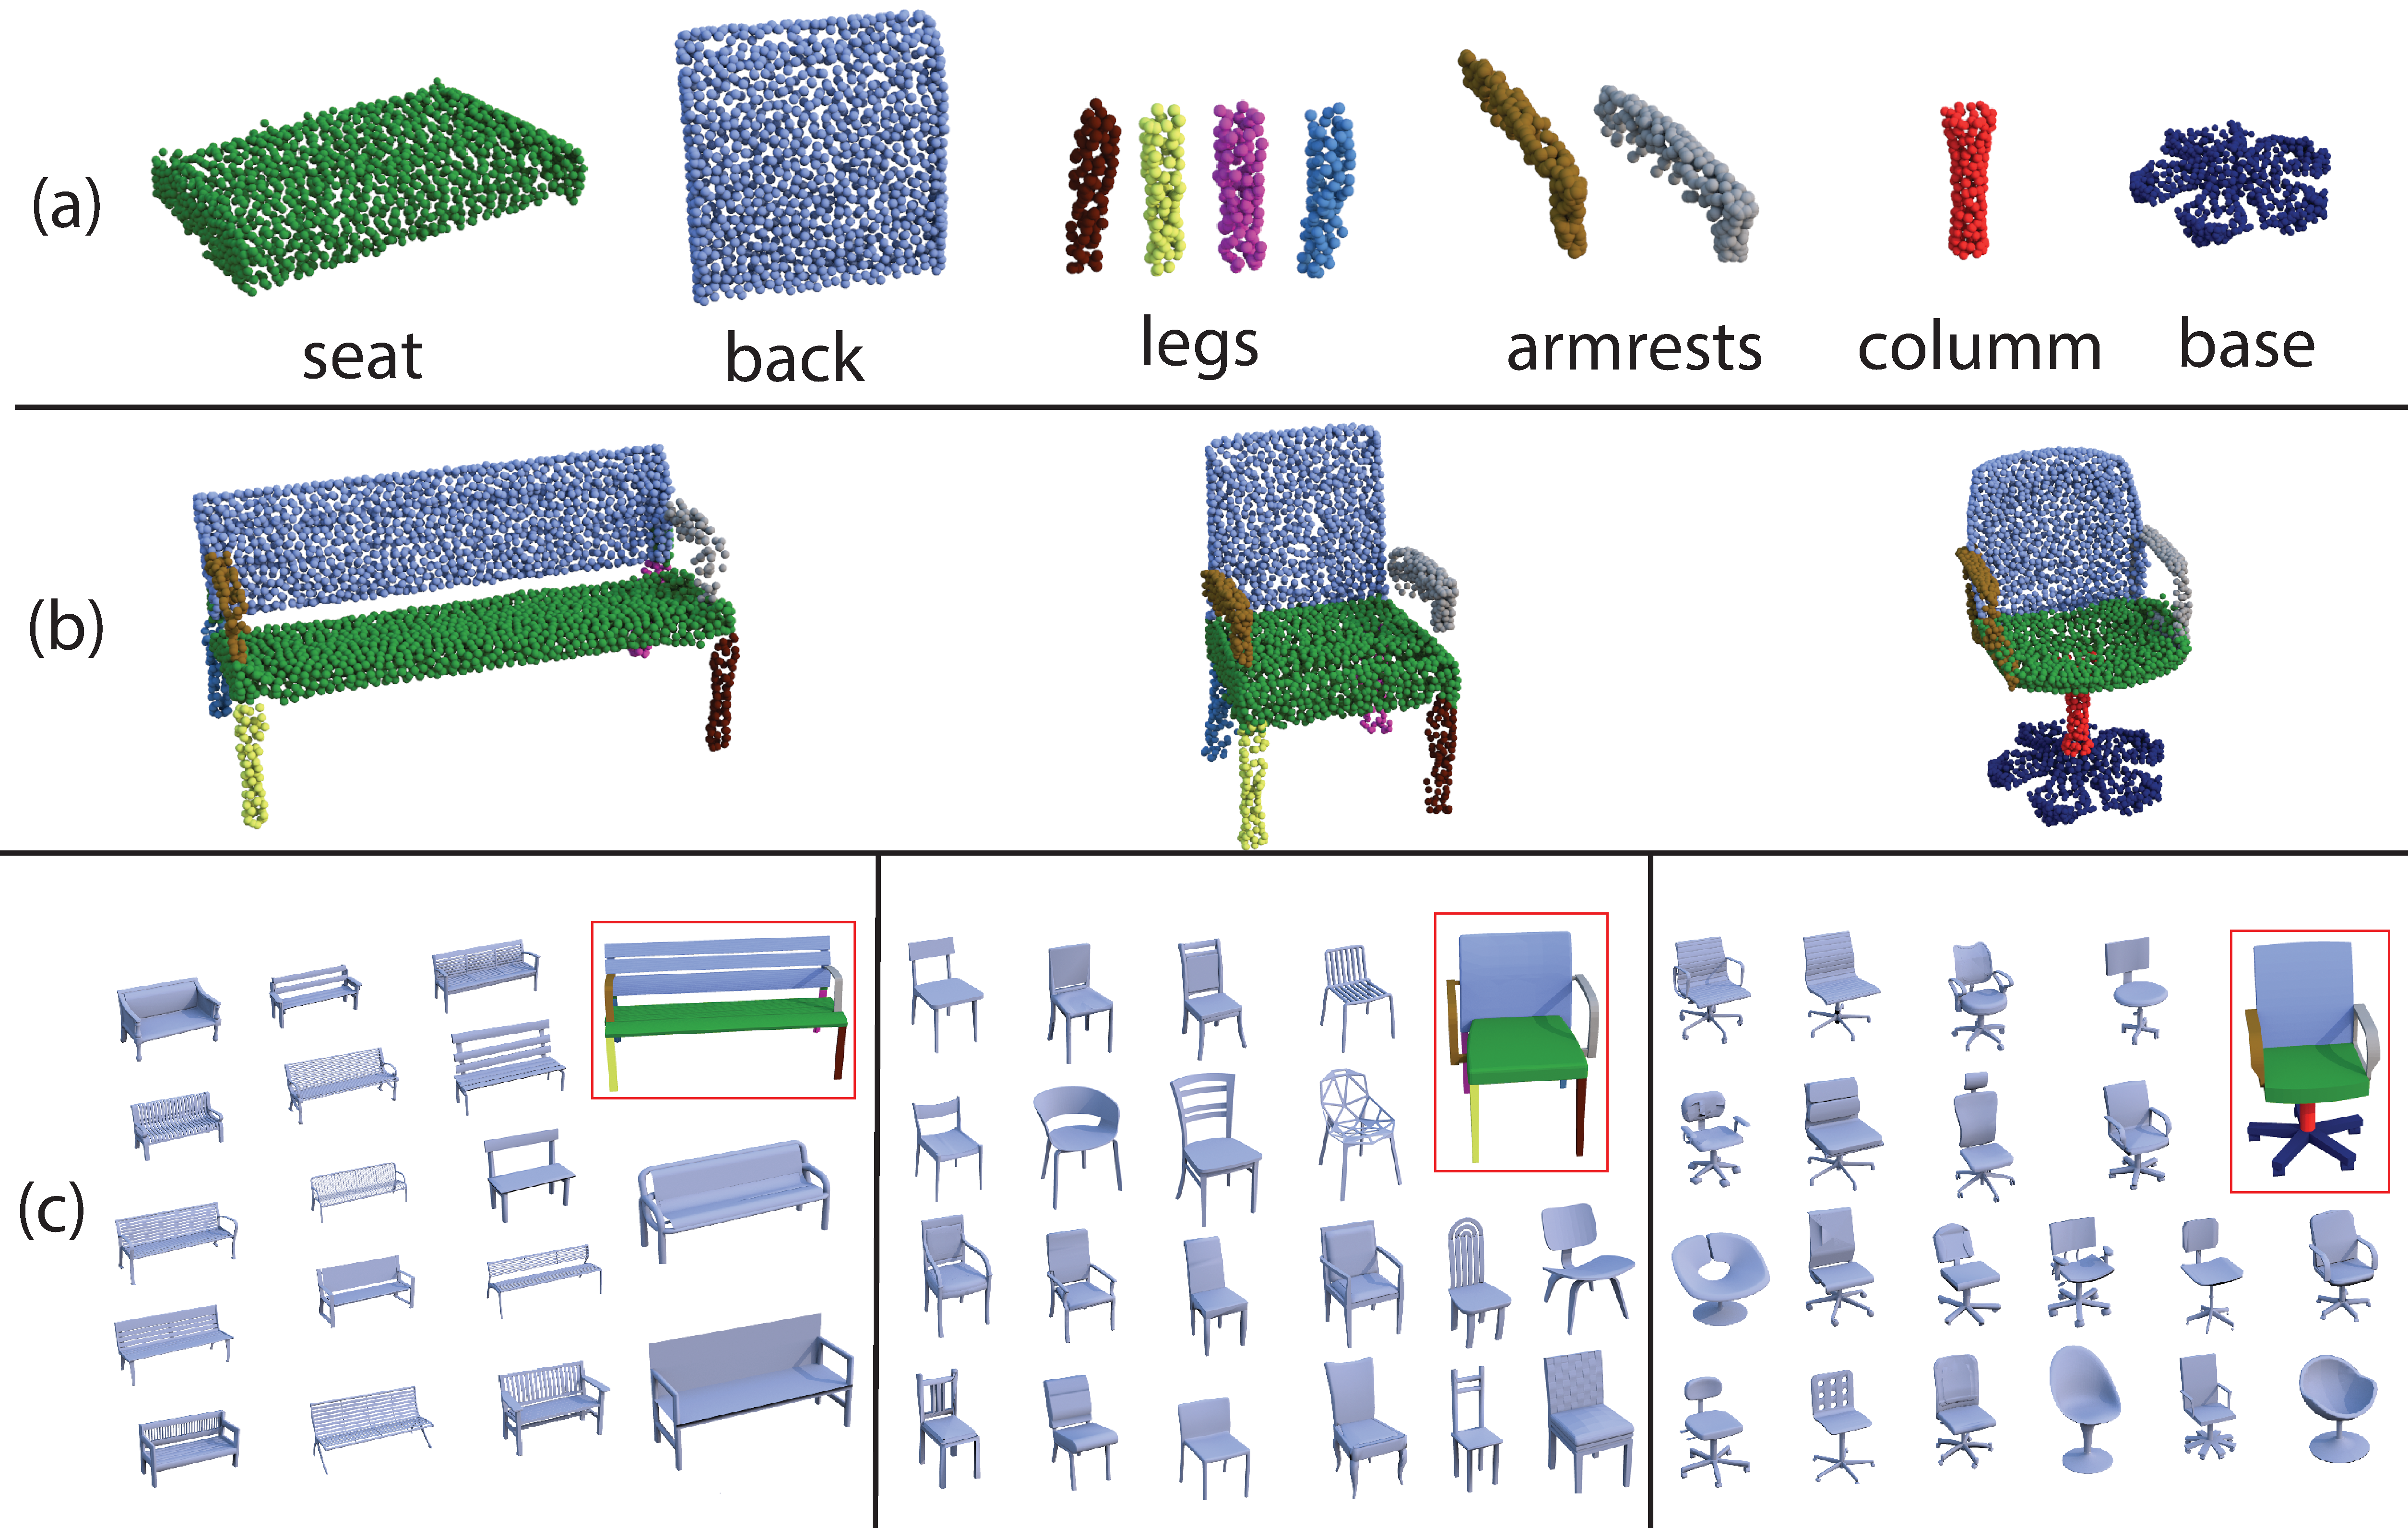
\includegraphics[width=1.0\columnwidth]{figures/hierarchy_learn}
\vskip -2mm
\caption{Hierarchical \rev{part template} learning for a collection of chairs. (a) Learned high-level \rev{part templates} for all chairs. (b) Learned \rev{part templates} per chair type or group (benches, four-legged chairs, office chairs). (c) Representative shapes per group and exemplar segmented shapes (in red box). }
\vskip -8mm
\label{fig:hierarchy}
\end{figure}

\textbf{Probabilistic deformation model.} At the heart of our algorithm lies a probabilistic deformation model (Section \ref{sec:part_representation_learning}). The model evaluates the probability of deformations applied on the \rev{part templates} under different corresponding point and part assignments over the input shape surfaces. By performing probabilistic inference on this model, our method iteratively computes the most likely deformation of the \rev{part templates} to match the input shape parts (Figure \ref{fig:deformation}). At each iteration, our method deforms the \rev{part templates}, and updates probabilities of point and part assignments over the input shape surfaces. The updated probabilistic point and part assignments iteratively guides the deformation and vice versa until convergence.

\textbf{Generative surface model.} Based on the estimated probability distributions over corresponding point and part assignments on all the input shapes of the collection, our method learns a probabilistic model characterizing the structural and surface variability within a shape family (Section \ref{sec:bsm}). The surface variability is encoded in the model through a joint probability distribution that captures relationships between parts and surface point locations within the shape family. For example, consider airplanes. The position of wingtips is strongly related to the positions of other points on the same wing (i.e., the overall wing geometry), as well as the part arrangement and surface geometry of the whole airplane. These complex relationships of points and parts in the shapes of a family are hierarchically captured through latent variables. The model contains a layer of latent variables whose assignments are associated with arrangements of surface points within the same part. Higher-level layers of latent variables progressively capture relationships between surface points belonging to different shape parts. The latent variables also capture dominant modes of surface point arrangements corresponding to structurally different shape groups. By sampling the latent variables on the top layer, our model can generate parts and surface points that are used to synthesize new shapes. \rev{The top layer also produces shape descriptors that can be used for fine-grained classification.} Through the captured relationships between point locations, the model can be used to further improve correspondences in the shapes of the collection. 

\textbf{Pre-processing.} Our method requires the following pre-processing, or initialization: first, we rely on the rigid alignments provided by Kim et al. \shortcite{Kim13} to consistently orient the input shapes of each collection. Practically, we found that our surface variability model can tolerate incorrectly aligned shapes in the collections (e.g. about 5\% of the input shapes were not aligned correctly in the dataset it was trained on). Second, our method requires as input a labeled segmentation for at least one shape per group (Figure \ref{fig:hierarchy}c, red boxes). The segmentation can be provided by either the user, or an automatic co-segmentation technique. In the case of manual input, to facilitate the user, our method automatically clusters the shapes into groups and selects an exemplar shape per group. The user is asked to segment these exemplar shapes. In the case of co-segmented input, we use the segmentations provided by Kim et al. \shortcite{Kim13}. We note that the provided segmentations are used for initialization only: given initial segments, our methods learns the \rev{part templates} and improves the shape segmentations. 

